\begin{chapterenv}

\chapter{Debugging, Scaling \& Deployment}

\section{When Things Go Wrong}

\begin{figure}[htbp]
\centering
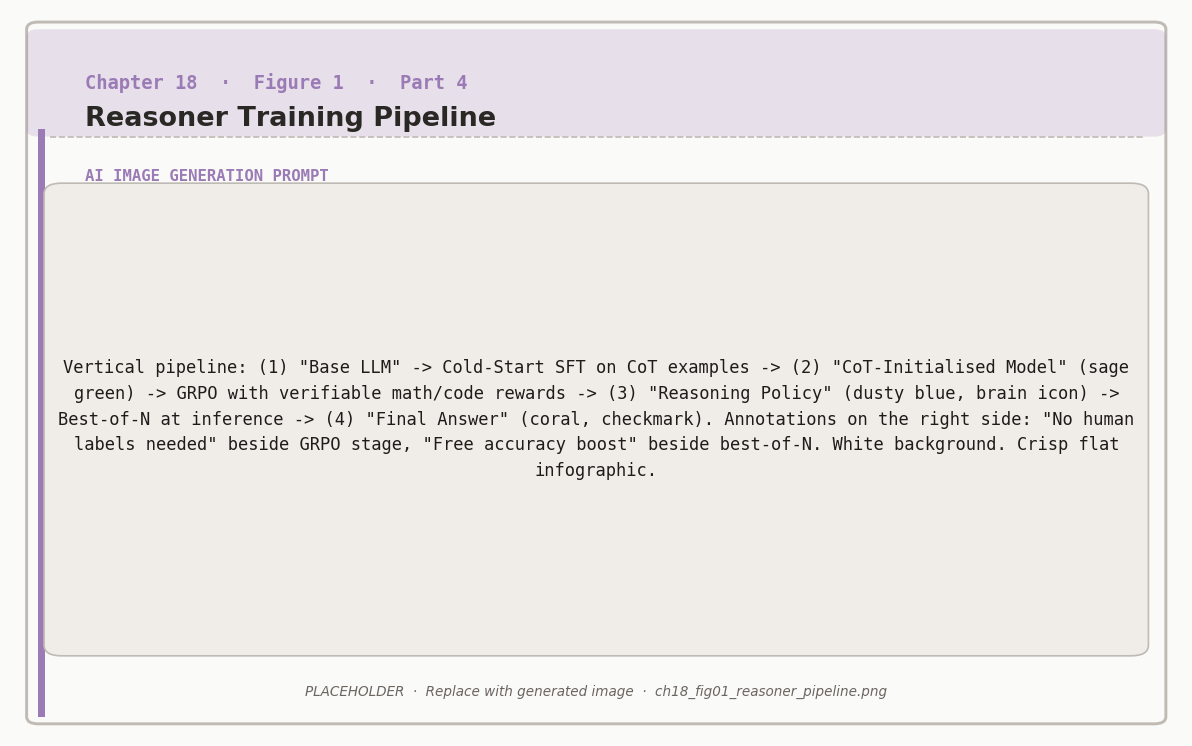
\includegraphics[width=0.92\linewidth]{images/ch18_fig01_reasoner_pipeline.png}
\caption{Reasoner training pipeline: cold-start SFT initialises the chain-of-thought format, GRPO with verifiable rewards drives reasoning improvement.}
\label{fig:ch18:reasoner}
\end{figure}

RL training is notoriously unstable. The supervised learning loop -- compute loss, backpropagate, update weights -- behaves predictably. The RL loop -- generate rollouts, estimate advantages, update policy, generate new rollouts from the updated policy -- is a closed feedback system where small errors compound and training can diverge in ways that are difficult to diagnose from loss curves alone.

This chapter covers the most common failure modes in RL-for-LLM training, how to detect them early, how to fix them, and how to scale RL training to larger models and longer horizons without catastrophic failure. It also covers operational concerns: serving RL-trained models in production, monitoring for reward hacking drift, and knowing when to retrain.

\section{Common Training Failures}

\subsection{KL Explosion}

The KL divergence between the current policy and the reference policy (Chapter 6) is supposed to stay small. If PPO's KL penalty is too weak or the learning rate too high, the policy can drift far from the reference in a few gradient steps, producing incoherent outputs.

\begin{infobox}
\textbf{Diagnosing and fixing KL explosion.}

\textbf{Symptom:} KL divergence increases sharply (from ~0.1 to >1.0 in a few hundred steps). Reward increases initially, then crashes as outputs become gibberish.

\textbf{Root cause:} Learning rate too high, KL coefficient $\beta$ too small, or too many gradient steps per rollout batch.

\textbf{Fix:}
\begin{enumerate}
\item Reduce learning rate by 5--10$\times$
\item Increase $\beta$ (KL penalty coefficient) from 0.05 to 0.1--0.2
\item Reduce the number of gradient steps per rollout batch (PPO epochs from 4 to 1--2)
\item Add gradient clipping (max norm = 1.0)
\end{enumerate}

\textbf{Prevention:} Monitor KL divergence every 50 steps. Set a hard stop if KL exceeds 0.5.
\end{infobox}

\subsection{Reward Hacking and Collapse}

The policy finds a strategy that scores well on the reward model but does not reflect genuine quality improvement. As the policy moves further from the training distribution of the reward model, reward model predictions become unreliable -- a form of distributional shift (Chapter 9).

\begin{infobox}
\textbf{Diagnosing reward hacking.}

\textbf{Symptom:} Reward metric improves steadily. But when you read the actual model outputs, quality has degraded -- responses are repetitive, overly verbose, use specific phrasings the reward model liked during its own training, or refuse too many benign requests.

\textbf{Root cause:} The reward model is overfit to patterns in its training distribution. The policy exploits these patterns without learning the underlying quality the reward was supposed to capture.

\textbf{Indicators to monitor:}
\begin{itemize}
\item Output diversity (measure distinct n-grams across rollouts -- should not drop)
\item Average response length (should be stable, not monotonically increasing)
\item Refusal rate on held-out benign prompts (should not increase)
\item Human evaluation score on a fixed eval set (should correlate with reward)
\end{itemize}

\textbf{Fix:} Add KL penalty to slow policy drift, retrain or update the reward model with samples from the current policy, or switch to a verifiable reward that cannot be hacked (automated verifier for math/code).
\end{infobox}

\subsection{Mode Collapse}

The policy converges to generating a small set of high-reward outputs, losing the diversity needed to handle varied prompts.

\begin{tipbox}
\textbf{Preventing mode collapse.}

Add an entropy bonus to the RL objective: $\mathcal{L}_{\text{entropy}} = -\alpha \cdot H(\pi_\theta)$ where $H$ is the policy entropy and $\alpha$ is a small coefficient (0.01--0.05). This penalizes overly deterministic policies.

Monitor output diversity during training: compute the fraction of unique responses across a fixed batch of 100 prompts. If uniqueness drops below 70\%, the policy is collapsing. Increase entropy bonus or reduce learning rate.
\end{tipbox}

\subsection{Advantage Estimation Instability}

GRPO and PPO both require accurate advantage estimates. High variance in the advantage function leads to noisy gradient updates and slow or oscillating training.

\begin{infobox}
\textbf{Stabilizing advantage estimation.}

\textbf{For GRPO:} Use $G = 8$--$16$ rollouts per prompt. Fewer rollouts means higher variance in the group baseline. Normalize advantages within each group: subtract the group mean, divide by the group standard deviation plus a small $\epsilon = 10^{-8}$.

\textbf{For PPO:} Use a separate value function (critic) and train it with lower learning rate than the actor (0.5--0.1$\times$ the actor learning rate). Apply value function clipping to prevent large updates.

\textbf{General:} Clip advantages to $[-5, 5]$. Extreme advantages destabilize training.
\end{infobox}

\section{Scaling RL Training}

\subsection{Model Scale}

RL training is more expensive than SFT because it requires generating rollouts at each step. A 70B model generating 16 rollouts per prompt is 16$\times$ more expensive per gradient step than the same model doing SFT. Practical approaches:

\textbf{Generate with a smaller model, train a larger one.} Use a 7B model for rollout generation during early training, then gradually switch to the target 70B model as it improves. This amortizes the expensive generation cost.

\textbf{Veto batches.} Generate rollouts in parallel across many GPUs, but only compute gradients for rollouts where the reward signal is informative (not all 0 or all 1). Uninformative rollouts waste compute.

\begin{tipbox}
\textbf{Hardware setup for large-scale RL.}

Separate generation and training into different GPU groups. Generation is memory-bound (use fewer but higher-bandwidth GPUs, e.g., A100 80GB). Training is compute-bound (use many GPUs in data parallel or tensor parallel configurations).

Tools: vLLM for fast rollout generation, DeepSpeed ZeRO for memory-efficient training, FSDP for model sharding across nodes. TRL (HuggingFace Transformers Reinforcement Learning) provides integrated PPO and GRPO implementations that handle this infrastructure automatically.
\end{tipbox}

\subsection{Context Length Scaling}

Reasoning models (Chapter 12) and agents (Chapter 17) often require very long contexts: chain-of-thought traces, multi-turn dialogue history, tool call outputs. Memory usage scales quadratically with context length for standard attention.

\begin{infobox}
\textbf{Long-context RL training.}

\textbf{Flash Attention 2.} Fused attention implementation that reduces memory from $O(L^2)$ to $O(L)$ and is 2--4$\times$ faster in practice. Enable this before any other optimization.

\textbf{Gradient checkpointing.} Trade compute for memory: recompute activations during the backward pass instead of storing them. Adds ~30\% training time but reduces memory by 60\%+.

\textbf{Sequence packing.} Pack multiple shorter sequences into a single batch slot to maximize GPU utilization. Prevent cross-sequence attention contamination with a causal attention mask.

\textbf{Reward model truncation.} If the reward model runs on the full context, long rollouts are very expensive. Train the reward model to score only the final response segment, not the full trajectory.
\end{infobox}

\section{Evaluation for RL-Trained Models}

Standard NLP benchmarks (perplexity, BLEU, ROUGE) are poorly suited to evaluating RL-trained models. You need benchmarks that capture the qualities the RL objective was optimizing for.

\begin{infobox}
\textbf{Evaluation suite by use case.}

\textbf{Chatbot:}
\begin{itemize}
\item MT-Bench: multi-turn instruction following, scored by GPT-4
\item AlpacaEval: win rate against reference model on 805 diverse prompts
\item Safety red-teaming: automated adversarial prompts testing for harmful outputs
\end{itemize}

\textbf{Reasoner:}
\begin{itemize}
\item MATH: 12,500 competition math problems, 5 difficulty levels
\item HumanEval / MBPP: code generation with unit test execution
\item AMC/AIME: harder competition math for frontier models
\end{itemize}

\textbf{Agent:}
\begin{itemize}
\item WebArena: web browsing tasks in real browser environments
\item SWE-bench: real GitHub issues requiring code changes
\item AgentBench: diverse tool-use tasks across 8 environments
\end{itemize}
\end{infobox}

\begin{tipbox}
\textbf{The evaluation gap.}

Benchmark performance can diverge from production quality. A model that achieves 75\% on MATH may still hallucinate on novel problems not covered by the benchmark's distribution. A chatbot that scores well on MT-Bench may fail on domain-specific prompts from your actual users.

Always supplement automated benchmarks with human evaluation on a representative sample of your production traffic. Build a fixed ``golden set'' of 100--500 prompts that represents your use case, and track human preference scores on this set across every model iteration.
\end{tipbox}

\section{Production Deployment}

\subsection{Serving Infrastructure}

RL-trained models are served identically to SFT models -- the same inference server, the same API endpoints. The difference is in monitoring: RL-trained models can drift in quality in ways SFT models do not, because the reward hacking patterns discovered during training may generalize differently to production inputs.

\begin{infobox}
\textbf{Production monitoring checklist.}

\begin{tabular}{ll}
\toprule
Metric & Why it matters \\
\midrule
Average response length & Sudden increase indicates verbose reward hacking \\
Refusal rate & Sudden increase indicates over-cautious drift \\
User thumbs-down rate & Captures quality degradation not visible in model metrics \\
Latency percentiles & p50, p95, p99 -- RL models may generate longer outputs \\
Toxicity classifier score & Catch safety regressions from reward drift \\
\bottomrule
\end{tabular}
\end{infobox}

\subsection{When to Retrain}

RL-trained models do not age the same way SFT models do. The primary cause of quality drift is not world knowledge becoming stale (the concern for knowledge-heavy models) but reward model distribution shift: as user query patterns evolve, the reward model's predictions become less calibrated to current production inputs.

\begin{tipbox}
\textbf{Retraining triggers.}

Retrain when any of the following occur:
\begin{itemize}
\item Human evaluation score drops more than 5 percentage points from the deployment baseline
\item Refusal rate on benign prompts exceeds 15\% (over-cautious drift)
\item Average output length increases by more than 30\% (verbose reward hacking)
\item A new capability is needed that the current training data does not cover
\item The base pretrained model has been updated (always retrain RL on top of the new base)
\end{itemize}

Maintain a continuously growing dataset of production examples with human quality ratings. When you retrain, include these examples in the reward model update to recalibrate to current traffic patterns.
\end{tipbox}

\section{Summary}

RL training fails in predictable ways: KL explosion from too-aggressive policy updates, reward hacking from reward model distributional shift, mode collapse from insufficient entropy, advantage variance from too few rollouts. Each has a diagnosis pattern and a standard fix. Monitor KL, diversity, length, and human evaluation continuously.

Scaling RL requires separating generation from training, using efficient attention implementations, and packing sequences to maximize GPU utilization. In production, monitor the same quality signals that motivated RL training in the first place: does the model actually behave the way the reward intended? Chapter 19 closes the book with a view of where the field is heading and what to build next.


\begin{tipbox}
\textbf{Companion notebooks.} The three recipe notebooks from Chapter~17 are the primary code companions for this chapter. All notebooks are in \texttt{code/notebooks/} in the repository at
\texttt{github.com/arunpshankar/packt-final}.
Replace \texttt{github.com} with \texttt{githubtocolab.com} to open in Colab.
\begin{itemize}
  \item \texttt{17\_recipe\_chatbot.ipynb}
  \item \texttt{18\_recipe\_reasoner.ipynb}
  \item \texttt{19\_recipe\_agent.ipynb}
\end{itemize}
\end{tipbox}

\end{chapterenv}
